% Preamble
    \documentclass[aspectratio=169]{beamer}
    \usepackage[utf8]{inputenc}
    % Import packages
        \usepackage{multimedia}
        \usepackage{hyperref}
        \usepackage{xcolor}
        \usepackage{graphicx}
        \usepackage{lipsum}
        \usepackage{ragged2e}
        \usepackage{graphicx}
        \usepackage{float}
        \usepackage{caption}
        \usepackage{subcaption}
    % Notes
        \usepackage{pgfpages}
        %\setbeameroption{show notes}
        %\setbeameroption{show notes on second screen=right}
    % Beamer theme
        \usetheme[progressbar=frametitle]{metropolis}
        \setbeamertemplate{frame numbering}[fraction]
        \definecolor{primary}{RGB}{245, 10, 10}
        \setbeamercolor{palette primary}{bg=white, fg=black}
        \setbeamercolor{background canvas}{parent=palette primary}
        \setbeamercolor{normal text}{fg=black}
        \setbeamercolor{progress bar}{use=palette primary,fg=primary}
    % Title page
        \title{Premios Nobel de Economía}
        \subtitle{Economía}
        \author[JR]{Jhon Roly (JR)}
        \institute{
            Universidad Nacional de San Cristóbal de Huamanga\\
            Facultad de Ciencias Económicas, Administrativas y Contables\\
            Escuela Profesional de Economía
        }
        \date{\today}
% Slides
\begin{document}
    % title
    \begin{frame}
        \titlepage
    \end{frame}
    % table of contents
    \begin{frame}{Contenido}
        \tableofcontents
    \end{frame}
    % Section 1
    \section{Introducción}
        \begin{frame}[t]{Introducción}
            \justify
            \begin{itemize}
                \item El Premio de Ciencias Económicas del Banco de Suecia en Memoria
                de Alfred Nobel, conocido popularmente como Premio Nobel de Economía
                es entregado anualmente por la Real Academia de las Ciencias de Suecia 
                y es una de las más importantes distinciones otorgadas a todos aquellos 
                intelectuales de la economía que han contribuido de manera favorable a 
                una teoría o actividad.
                \item Es entregado por la Real Academia de las Ciencias de Suecia, en Estocolmo.
                \item Este premio, a diferencia de los otros cinco que llevan su nombre, no fue 
                creado por Alfred Nobel, sino que se comenzó a entregar en 1969 por iniciativa 
                y con recursos del Banco de Suecia, con la denominación de Premio de Ciencias 
                Económicas del Banco de Suecia en Memoria de Alfred Nobel, con el consentimiento 
                y bajo la administración de la Fundación Nobel.
                \item El ganador del premio recibe 10 millones de coronas suecas, alrededor de 
                1.1 millones de euros, una medalla de oro y un diploma.
            \end{itemize}
        \end{frame}   
    % Section 2
    \section{Gandores del Premio Nobel}
        % 1969
        \begin{frame}[t]{1969}
            \justify
            Por desarrollar y aplicar los modelos dinámicos para el análisis de los procesos económicos
            \begin{figure}[ht]
                \centering
                \caption{Ganadores del Premio Nobel de Economía en 1969}
                \begin{subfigure}[b]{0.49\textwidth}
                    \centering
                    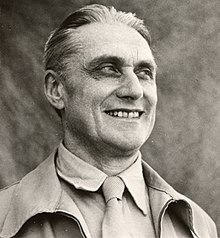
\includegraphics[scale = 0.4]{ImgEconomy/RagnarFrisch.jpg}
                    \caption{Ragnar Frisch\footnote{Países Bajos}}
                    \label{fig: RagnarFrisch}
                \end{subfigure}
                \hfill 
                \begin{subfigure}[b]{0.49\textwidth}
                    \centering
                    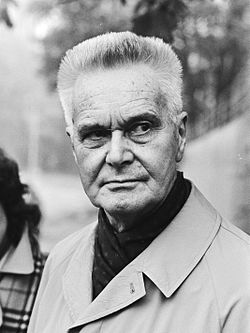
\includegraphics[scale = 0.3]{ImgEconomy/JanTinbergen.jpg}
                    \caption{Jan Tinbergen\footnote{Noruega}}
                    \label{fig: JanTinbergen}
                \end{subfigure}
                \label{fig: Ganadores1969}
            \end{figure}
        \end{frame}
        % 1970
        \begin{frame}[t]{1970}
            \justify
            Por el trabajo científico a través del cual ha desarrollado una teoría para la economía, 
            estática y dinámica, contribuyendo a elevar el nivel de análisis en la ciencia económica.
            \begin{figure}[ht]
                \centering
                \caption{Ganador del Premio Nobel de Economía en 1970}
                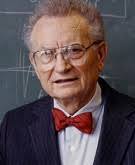
\includegraphics[scale = 0.55]{ImgEconomy/PaulSamuelson.jpg}
                \caption*{Paul Samuelson\footnote{Estados Unidos}}
                \label{fig: PaulSamuelson}
            \end{figure}
        \end{frame}
        % 1971
        \begin{frame}[t]{1971}
            \justify
            Por su interpretación empíricamente fundada del crecimiento económico, que ha llevado 
            a un nuevo y más profundo acercamiento a la estructura económica y social y a los 
            procesos de desarrollo.
            \begin{figure}[ht]
                \centering
                \caption{Ganador del Premio Nobel de Economía en 1971}
                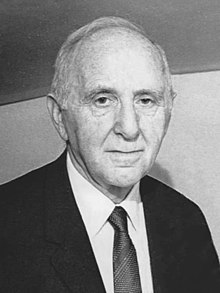
\includegraphics[scale = 0.27]{ImgEconomy/SimonKuznets.jpg}
                \caption*{Simon Kuznets\footnote{Estados Unidos}}
                \label{fig: SimonKuznets}
            \end{figure}
        \end{frame}
        % 1972
        \begin{frame}[t]{1972}
            \justify
            Por sus contribuciones a la teoría del equilibrio económico y del bienestar.
            \begin{figure}[ht]
                \centering
                \caption{Ganadores del Premio Nobel de Economía en 1972}
                \begin{subfigure}[b]{0.49\textwidth}
                    \centering
                    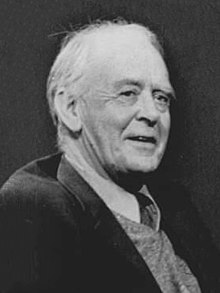
\includegraphics[scale = 0.35]{ImgEconomy/JohnHicks.jpg}
                    \caption{John Hicks\footnote{Reino Unido}}
                    \label{fig: JohnHicks}
                \end{subfigure}
                \hfill 
                \begin{subfigure}[b]{0.49\textwidth}
                    \centering
                    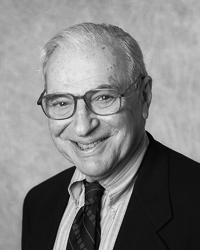
\includegraphics[scale = 1.7]{ImgEconomy/KennethArrow.jpg}
                    \caption{Kenneth Arrow\footnote{Estados Unidos}}
                    \label{fig: KennethArrow}
                \end{subfigure}
                \label{fig: Ganadores1972}
            \end{figure}
        \end{frame}
        % 1973
        \begin{frame}[t]{1973}
            
        \end{frame}
        % 1974
        % 1975
        % 1976
        % 1977
        % 1978
        % 1979
        % 1980


    % Source : https://es.wikipedia.org/wiki/Portal:Premios_Nobel/Premio_Nobel_de_Econom%C3%ADa
    
\end{document}